\section{常见接口} 

\subsection{SPI}
SPI是很多术语的缩写。包括:
\subsubsection{serial peripheral interface}
序列周边接口(Serial Peripheral Interface Bus,SPI),类似I²C,是一种4线同步序列资料协定,适用于可携式装置平台系统,但使用率较I²C少。序列周边接口一般是4线,有时亦可为3线,有别于I²C的2线,以及1-Wire。

The Serial Peripheral Interface Bus or SPI (pronounced as either ess-pee-eye, spy or simply S.P.I) bus is a synchronous serial data link standard, named by Motorola, that operates in full duplex mode. Devices communicate in master/slave mode where the master device initiates the data frame. Multiple slave devices are allowed with individual slave select (chip select) lines. Sometimes SPI is called a four-wire serial bus, contrasting with three-, two-, and one-wire serial buses.
\subsubsection{System Packet Interface}
The System Packet Interface family of Interoperability Agreements from the Optical Internetworking Forum specify chip-to-chip, channelized, packet interfaces commonly used in synchronous optical networking and ethernet applications. A typical application of such a packet level interface is between a framer (for optical network) or a MAC (for IP network) and a network processor. Another application of this interface might be between a packet processor ASIC and a traffic manager device.

SPI-4.2 is a version of the System Packet Interface published by the Optical Internetworking Forum. It was designed to be used in systems that support OC-192 SONET interfaces and is sometimes used in 10 Gigabit Ethernet based systems.
SPI-4 is an interface for packet and cell transfer between a physical layer (PHY) device and a link layer device, for aggregate bandwidths of OC-192 Asynchronous Transfer Mode(ATM) and Packet over SONET/SDH (POS), as well as 10 Gigabit Ethernet applications.
A typical application of SPI-4.2 is to connect a framer device to a network processor. It has been widely adopted by the high speed networking marketplace.
The clocking is Source-synchronous and operates around 700 MHz. Implementations of SPI-4.2 have been produced which allow somewhat higher clock rates. This is important when overhead bytes are added to incoming packets.






\subsection{I2C}
I²C(Inter-Integrated Circuit)是内部整合电路的称呼,是一种串行通讯总线,使用多主从架构,由飞利浦公司在1980年代为了让主板、嵌入式系统或手机用以连接低速周边装置而发展。I²C的正确读法为``I-squared-C'' ,而``I-two-C''则是另一种错误但被广泛使用的读法,在中国则多以``I方C''称之。截至2006年11月1日为止,使用I²C协定不需要为其专利付费,但制造商仍然需要付费以获得I²C从属装置位址。


原始的I²C系统是在1980年代所建立的一种简单的内部总线系统,当时主要的用途在于控制由飞利浦所生产的芯片。
1992年完成了最初的标准版本释出,新增了传输速率为400 kbit/s的快速模式及长度为10位元的寻址模式可容纳最多1008个节点。1998年释出了2.0版,新增了传输速率为3.4Mbit/s的高速模式并为了节省能源而减少了电压及电流的需求。2.1版则在2001年完成,这是一个对2.0版做一些小修正,version 3.0, 2007年同时也是目前的最新版本。

在Linux中,I²C已经列入了核心模组的支援了,更进一步的说明可以参考核心相关的文件及位于/usr/include/linux/i2c.h 的这个标头档。OpenBSD则在最近的更新中加入了I²C的架构(framework)以支援一些常见的主控端控制器及感应器。

\subsection{UEXT}
Universal EXTension (UEXT) is a connector layout which includes power and three serials buses: Asynchronous, I2C, SPI. The connector layout was specified by Olimex Ltd and declared an open-project that is royalty-free.

\subsection{PCI}
外设互联标准(或称个人电脑接口,Personal Computer Interface),实际应用中简称为PCI(Peripheral Component Interconnect),是一种连接电子计算机主板和外部设备的总线标准。一般PCI设备可分为以下两种形式:
直接布放在主板上的集成电路,在 PCI 规范中称作“平面设备”(planar device);或者
安装在插槽上的扩展卡。
PCI bus常见于现代的个人计算机中,并已取代了ISA和VESA 局部总线,成为了标准扩展总线。PCI 总线亦常见于其他电子计算机类型中。PCI总线最终将被PCI Express和其他更先进的技术取代,这些技术现在已经被用于最新款的电子计算机中。
PCI 规范规定了该总线的物理尺寸(包括线宽)、电气特性、总线时序和协议。该规范可从美国PCI-SIG协会购得。
常见的PCI卡包括网卡、声卡、调制解调器、电视卡和磁盘控制器,还有USB和串口等端口。原本显卡通常也是PCI设备,但很快其带宽已不足以支持显卡的性能。PCI显卡现在仅用在需要额外的外接显示器或主板上没有AGP和PCI Express槽的情况。

\subsection{MII}
MII(Media Independent Interface,媒体独立接口),是与100Mbps的Ethernet PHY chip沟通时所使用的接口。

Being media independent means that different types of PHY devices for connecting to different media (i.e. Twisted pair copper, fiber optic, etc.) can be used without redesigning or replacing the MAC hardware. Thus any MAC may be used with any PHY, independent of the network signal transmission media.The MII can be used to connect a MAC to an external PHY using a pluggable connector, or direct to a PHY chip which is on the same printed circuit board.On a PC the CNR connector Type B carries MII bus interface signals.The MDIO Serial Management Interface (SMI) (see MDIO) is used to transfer management information between MAC and PHY.

Reduced Media Independent Interface (RMII) is a standard that addresses the connection of Ethernet physical layer transceivers (PHY) to Ethernet switches or the MAC portion of an end-device's Ethernet interface. It reduces the number of signals/pins required for connecting to the PHY from 16 (for an MII-compliant interface) to between 6 and 10. RMII is capable of supporting 10 and 100 Mbit/s; even 1 Gbit/s is possible, higher gigabit interfaces need a wider interface.

An Ethernet interface normally consists of 4 major parts: The MAC (Media Access Controller), the PHY (PHYsical Interface or transceiver), the magnetics, and the connector.

RMII is one of the possible interfaces between the MAC and PHY; others include MII and SNI, with additional wider interfaces (including XAUI, GBIC, SFP, SFF, XFP, and XFI) for gigabit and faster Ethernet links.

Gigabit Media Independent Interface (GMII) is an interface between the Media Access Control (MAC) device and the physical layer (PHY). The interface defines speeds up to 1000 Mbit/s.

RGMII uses half the number of data pins as used in the GMII interface. This reduction is achieved by clocking data on both the rising and falling edges of the clock in 1000 Mbit/s operation, and by eliminating non-essential signals.

The Serial Gigabit Media Independent Interface (SGMII) is a variant of MII, a standard interface used to connect an Ethernet MAC-block to a PHY. It is used for Gigabit Ethernet but can also carry 10/100 MBit Ethernet.

10 Gigabit Media Independent Interface (XGMII) is a standard defined in IEEE 802.3 for connecting full duplex 10 Gigabit Ethernet (10GbE) ports to each other and to other electronic devices on a printed circuit board.

XAUI是一个介于MAC到PHY之间电脑总线XGMII(10.0 Gbit/s)的延伸标准,XAUI发音``zowie'',与意味十倍的罗马数字 X 关联,是“附件单位接口”的起始。
XAUI是XGMII的延伸,XAUI位于MAC末端的XGXS、和PHY末端的XGXS之间。XAUI延伸了XGMII的操作长度并减少了信号接口的数目。应用范围包括延伸MAC和PHY模组之间的实体分隔以10.0 Gbit/s 以太系统分散横跨电路板。

The XGMII Extender, which is composed of an XGXS(The 10 Gigabit Ethernet Extended Sublayer) at the MAC end, an XGXS at the PHY end and a XAUI between them, is to extend the operational distance of the XGMII and to reduce the number of interface signals. Applications include extending the physical separation possible between MAC and PHY components in a 10 Gigabit Ethernet system distributed across a circuit board.


在10Mbps 以太网上,对应的是AUI, Attachment Unit Interface。

The MII design has been extended to support reduced signals and increases speeds. Current variants are Reduced Media Independent Interface, Gigabit Media Independent Interface, Reduced Gigabit Media Independent Interface, Serial Gigabit Media Independent Interface and 10 Gigabit Media Independent Interface.

\subsection{PCI-E}
PCI Express,简称PCI-E,是电脑总线PCI的一种,它沿用了现有的PCI编程概念及通讯标准,但建基于更快的串行通信系统。英特尔是该接口的主要支援者。PCIe仅应用于内部互连。由于PCIe是基于现有的PCI系统,只需修改物理层而无须修改软件就可将现有PCI系统转换为PCIe。PCIe拥有更快的速率,以取代几乎全部现有的内部总线(包括AGP和PCI)。英特尔希望将来能用一个PCIe控制器和所有外部设备交流,取代现有的南桥/北桥方案。

除了这些,PCIe设备能够支援热拔插以及热交换特性,支援的三种电压分别为+3.3V、3.3Vaux以及+12V。考虑到现在显卡功耗的日益增加,PCIe而后在规范中改善了直接从插槽中取电的功率限制,16x的最大提供功率达到了75W[1],比AGP 8X接口有了很大的提升。基本可以满足当时(2004年)中高阶显卡的需求。这一点可以从AGP、PCIe两个不同版本的6600GT显卡上就能明显地看到,后者并不需要外接电源。PCIe只是南桥的扩展总线,它与操作系统无关,所以也保证了它与原有PCI的兼容性,也就是说在很长一段时间内在主板上PCIe接口将和PCI接口共存,这也给用户的升级带来了方便。由此可见,PCIe最大的意义在于它的通用性,不仅可以让它用于南桥和其他设备的连接,也可以延伸到芯片组间的连接,甚至也可以用于连接图形芯片,这样,整个I/O系统重新统一起来,将更进一步简化计算机系统,增加计算机的可移植性和模块化。

\section{主板结构}

\subsection{芯片组}
芯片组(chipset, PC chipset, or chip set)是一组共同工作的集成电路(“芯片”),并作为一个产品销售。它负责将电脑的核心——微处理器和机器的其他部分相连接,是决定主板级别的重要部件。以往,芯片组由多颗芯片组成,慢慢的简化为两颗芯片。

在计算机领域,“芯片组”术语通常是特指计算机主板或扩展卡上的芯片,如图\ref{fig:chipset}所示。当讨论基于英特尔的奔腾级处理器的个人电脑时,芯片组一词通常指两个主要的主板芯片组:北桥和南桥。芯片组的制造商可以,通常也是独立于主板的制造商。比如PC主板芯片组包括NVIDIA的nForce芯片组和威盛电子公司的KT880,都是为AMD处理器开发的,或英特尔许多芯片组。
\begin{figure}[ht]
	\begin{center}
		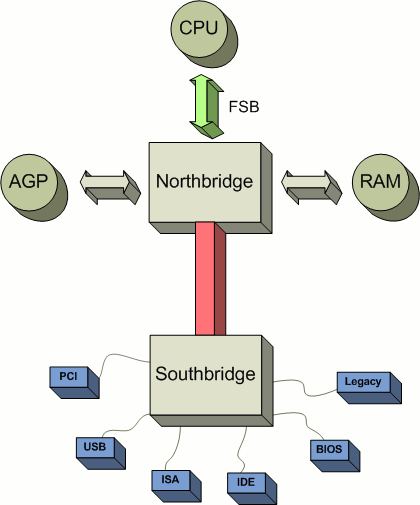
\includegraphics[keepaspectratio,width=0.5\paperwidth]{Pictures/Schema_chipsatz.png}
	\end{center}
	\caption{主板芯片组}
	\label{fig:chipset}
\end{figure}

单芯片芯片组已推出多年,例如SiS 730。但直到最近nForce 4的出现才逐渐流行。现在的单芯片芯片组,不像以往般复杂,因Athlon 64已内建内存控制器,取代了北桥的功能。纵使芯片组变成单芯片,习惯上亦沿用旧名称。

北桥(英语:Northbridge)是基于Intel处理器的个人电脑主板芯片组两枚芯片中的一枚,北桥设计用来处理高速信号,通常处理中央处理器、随机存取存储器、AGP或PCI Express的端口,还有与南桥之间的通信。


传统的北桥内建内存控制器,让处理器连接前端总线,而处理器和内存总线则跑相同的时脉。随后,芯片组分开处理器和内存总线的频率,让前端总线只代表处理器和北桥之间的通道。

北桥留下来的只剩下AGP或PCI Express控制器和与南桥通信,有时北桥会和南桥整合在同颗芯片中,有一些北桥则连绘图处理器也整合进去,而另外支援AGP或PCI Express接口。整合式北桥会侦测到附加在AGP插槽上有安装显卡,并停止其绘图处理器功能,但有些北桥可以允许同时使用整合式显卡和安装外加显卡,作为多显示输出。

Intel Hub Architecture(IHA)可用来取代南桥与北桥,IHA芯片组亦分成二大项:Graphics和AGP Memory Controller Hub (GMCH)与I/O Controller Hub (ICH)。

AMD在Athlon 64时代将内存总线整个拿掉,直接设计到处理器中,让北桥的功能只是支援外加显卡接口,例如AGP和PCI Express x16。由于北桥的重要性降低,有厂商索性将南北桥合并,成为单一芯片组,例如NVIDIA的nForce 4。这样可以减低芯片组的制造成本,但电脑的效能会降低。

南桥是基于Intel处理器的个人电脑主板芯片组两枚芯片中的一枚。南桥设计用来处理低速信号,通过北桥与CPU联系。各芯片组厂商的南桥名称都有所不同,例如英特尔称之为ICH,NVIDIA的称为MCP,ATI的称为IXP/SB。

南桥包含大多数周边设备接口、多媒体控制器和通讯接口功能。例如PCI控制器、ATA控制器、USB控制器、网络控制器、音效控制器。各世代的南桥效能大多雷同,但偶然听到某些南桥会有较差的Serial ATA或USB效能。

目前所有的南桥制造商都提供SATA磁盘阵列功能,NVIDIA则允许SATA和ATA硬盘机混合组成磁盘阵列。最新的英特尔Matrix RAID技术,让RAID-0和RAID-1组态可以在两颗硬盘机中同时使用。

大多数南桥都能直接连接Gigabit Lan PHY(实体层芯片,用来处理连接讯号),高阶的南桥通常拥有两组Gigabit Lan PHY,不过中阶的主板则只支援一组。而NVIDIA最新的南桥则支援带宽合并、封包排序和TCP/IP加速等高级网络卡功能。现在大部份高级南桥则支援Azalia高传真音效,借着编码芯片支援7.1声道音效。

大多数南桥都支援PCI Express Hub,但主板制造商通常采用北桥所提供的PCI Express Lane。
\subsection{前端总线}
前端总线(FSB,Front Side Bus)是指中央处理器数据总线的专门术语,此总线负责中央处理器和北桥芯片间的数据传递。如图\ref{fig:mainboard}。

\begin{figure}[htb]
\centering
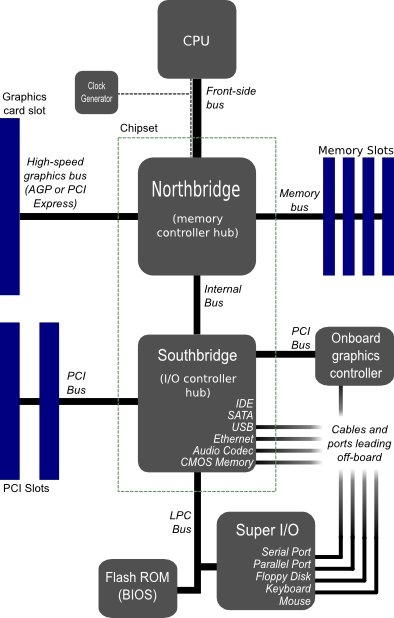
\includegraphics[keepaspectratio,width=0.5\paperwidth]{Pictures/Motherboard_diagram.jpg}
\caption{典型的PC主板}
\label{fig:mainboard}
\end{figure}
某些带有L2和L3缓存(Cache)的计算机,通过后端总线(Back Side Bus)实现这些缓存和中央处理器的连接,而此总线的数据传输速率总是高于前端总线。

大多数现代总线(GTL+和EV6)是CPU和芯片组的连接主干。芯片组(通常由南桥和北桥组成)是和系统中其他总线的连接节点。PCI、AGP和内存总线均和芯片组相连,以使设备间数据能相互传送。

这些第二级系统总线的运行速率取决于前端总线的速率。总之,高的前端总线速率意味着计算机的高处理性能。

在PC发展初期,由于处理器速度不高,大部份元件的时脉均保持同步,直至80486时代,在处理器制程持续进步下,处理器速度也加速成长,当时由于其他外部元件受电气结构所限,而无法跟进成长,因此Intel首次于处理器时脉中加入倍频设计,首颗处理器为Intel 80486DX2,外部传输时脉是处理器的一半,及后处理器成长速度仍远超过外部元件,两者速度差距越来越大。直至Pentium III时代,处理器时脉已超越1GHz,但外部传输时脉仍仅有133MHz。

正常来说,外频速度越高代表处理器在同一周期下可读写越多的数据,因此,外频速度很可能会变成系统效能上的瓶颈,为解决处理器带宽不足的问题,Intel于Pentium 4时代加入Quad Pumped Bus架构,使其在同一周期内可传送4笔数据,此举令外部传输时脉不变下,传输效率却可提升四倍。

\subsection{内频与总线速率}
中央处理器的时脉速度(简称内频)由系统总线速率(bus speed)乘上倍频系数决定。例如,一个时脉速度为 700MHz 的处理器,可能运行于 100MHz 的系统总线上。这说明处理器内的时钟倍频器的倍率设置为7,即中央处理器被设定为以7倍于系统总线的速率运行:100 MHz×7 = 700 MHz。通过改变倍频系数或系统总线速率,可以得到不同的时脉速度。以前经常套用的规则认为:时脉速度=外频(前端总线、FSB)*倍频系数。这句话严格来说并不正确。因为现在系统总线、前端总线(外频、FSB)速率不一样。就 Intel CPU 来说,前端总线=系统总线*4。所以,应该说时脉速度=系统总线*倍频系数。大多数主板允许用户通过跳线设置(BIOS)设定倍频或系统总线速率。现在许多处理器制造商预先锁定了处理器的倍频,但可以通过某些手段解锁。对所有的处理器,系统总线速率的适当提高可以增进其处理速率。

系统总线(BusSpeed)与前端总线(FSB、外频)的区别在于,前端总线(FSB、外频)的速度指的是CPU和北桥芯片间总线的速度。而系统总线(BusSpeed)的概念是建立在数位脉冲信号震荡速度基础之上的,也就是说,100MHz系统总线(BusSpeed)特指数位脉冲信号在每秒钟震荡一百万次,它更多的影响了PCI及其他总线的频率。之所以前端总线(FSB、外频)与系统总线(BusSpeed)这两个概念容易混淆,主要的原因是在以前的很长一段时间里,前端总线(FSB、外频)与系统总线(BusSpeed)是相同速率,因此往往直接称系统总线(BusSpeed)为外频,最终造成这样的误会。随着电脑技术的发展,人们发现前端总线频率(外频、FSB)需要高于系统总线(BusSpeed),因此采用了QDR(Quad Date Rate)技术,或者其他类似的技术实现这个目的。这些技术的原理类似于AGP的2X或者4X,它们使得的前端总线(FSB、外频)频率成为系统总线(BusSpeed)的2倍、4倍甚至更高,从此之后系统总线(BusSpeed)和前端总线(FSB、外频)的区别才开始被人们重视起来。



\subsection{HyperTransport}

HyperTransport技术,简称“HT总线”,以前曾被称作“闪电数据传输”(Lightning Data Transport,LDT),是一种高速、双向、低延时、点对点的、串行或者并行的高带宽连接总线技术,于2001年4月2日开始投入使用。旨在提高个人计算机、服务器、嵌入式系统,以及网络和电信设备内集成电路之间的通信速度。该技术有助于减少系统之中的布线数量,从而能够减少系统瓶颈,让当前速度更快的微处理器能够更加有效地在高端多处理器系统中使用系统内存。由HyperTransport联合会(The HyperTransport Consortium)负责改进和发展此技术。AMD和全美达公司把这项技术应用在x86处理器上,而PMC-Sierra、Broadcom(博通)和Raza Microelectronics则把它应用在MIPS(一种RISC微处理器架构)微处理器上;除微处理器应用之外,AMD、NVIDIA、VIA和SiS把它用于PC主板的芯片组;惠普、Sun Microsystems、IBM、和IWill把它用于服务器领域;Cray、Newisys、 和QLogic把它用于高性能计算;CISCO Systems(思科)把它用于路由器领域。应该引起关注的是以上名单中唯独少了半导体巨头Intel,它继续选择使用一种共享的总线架构,但在Intel新的Nehalem架构(如Core i7)中内置了内存控制器。


具体应用有:
\begin{description}
	\item[替代前端总线]The primary use for HyperTransport is to replace the front-side bus, which is currently different for every type of machine. For instance, a Pentium cannot be plugged into a PCI Express bus. To expand the system, the proprietary front-side bus must connect through adapters for the various standard buses, like AGP or PCI Express. These are typically included in the respective controller functions, namely the northbridge and southbridge.

		In contrast, HyperTransport is an open specification, published by a multi-company consortium. A single HyperTransport adapter chip will work with a wide spectrum of HyperTransport enabled microprocessors. For example, Broadcom HT-1000 and HT-2000 server controller devices can work with many different HyperTransport enabled microprocessors.

		AMD uses HyperTransport to replace the front-side bus in their Opteron, Athlon 64, Sempron 64, Turion 64, Phenom, Phenom II and FX families of microprocessors.
	\item[多处理器]Another use for HyperTransport is as an interconnect for NUMA multiprocessor computers. AMD uses HyperTransport with a proprietary cache coherency extension as part of their Direct Connect Architecture in their Opteron and Athlon 64 FX (Dual Socket Direct Connect (DSDC) Architecture) line of processors. The HORUS interconnect from Newisys extends this concept to larger clusters. The Aqua device from 3Leaf Systems virtualizes and interconnects CPUs, memory, and I/O.
	\item[路由器和交换机]
	\item[协处理器连接]
	\item[扩展设备]
\end{description}


\begin{figure}[htb]
\centering
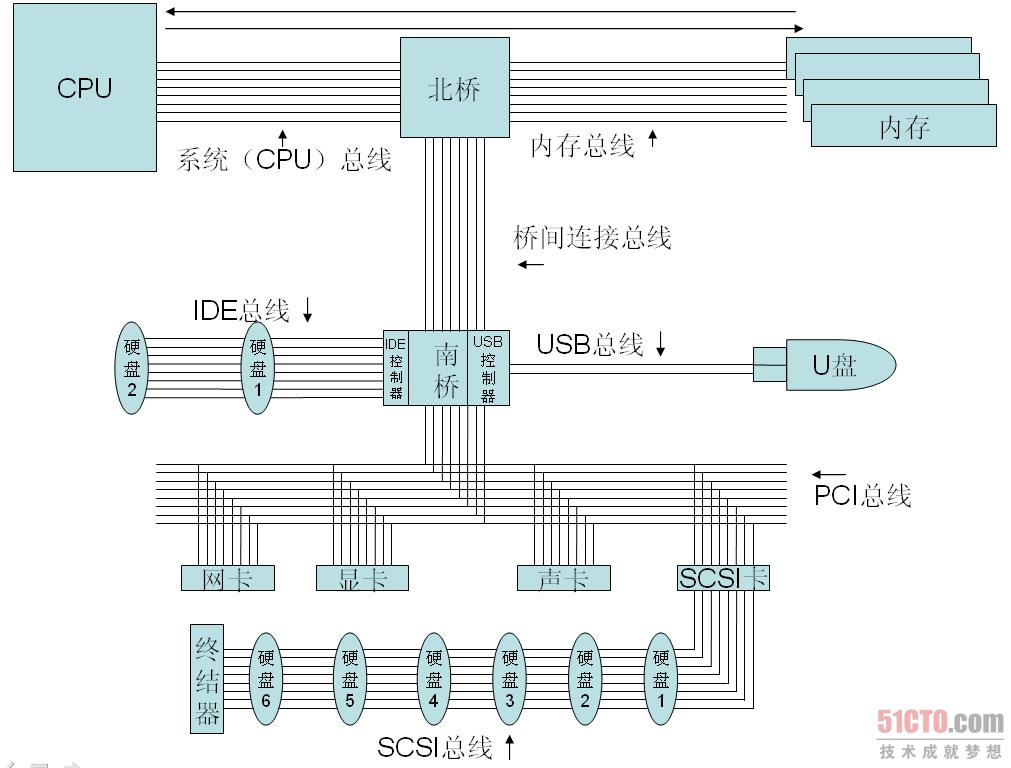
\includegraphics[keepaspectratio,width=0.5\paperwidth]{Pictures/g.jpg}
\caption{计算机总线图}
\label{fig:computerbuspic}
\end{figure}


\subsection{已过时的CNR插槽}
Communications and Networking Riser (CNR) is a slot found on certain PC motherboards and used for specialized networking, audio, and telephony equipment. A motherboard manufacturer can choose to provide audio, networking, or modem functionality in any combination on a CNR card. CNR slots were once commonly found on Pentium 4-class motherboards, but have since been phased out in favor of on-board or embedded components.














\section{OC速率}
Optical Carrier transmission rates are a standardized set of specifications of transmission bandwidth for digital signals that can be carried on Synchronous Optical Networking (SONET) fiber optic networks. Transmission rates are defined by rate of the bitstream of the digital signal and are designated by hyphenation of the acronym OC and an integer value of the multiple of the basic unit of rate, e.g., OC-48. The base unit is 51.84 Mbit/s. Thus, the speed of optical-carrier-classified lines labeled as OC-n is n × 51.84 Mbit/s.


\section{硬件测试相关知识}
\subsection{JTAG}
JTAG是联合测试工作组(Joint Test Action Group)的简称,是在名为标准测试访问端口和边界扫描结构的IEEE的标准1149.1的常用名称。此标准用于测试访问端口,使用边界扫描的方法来测试印刷电路板。

1990年JTAG正式由IEEE的1149.1-1990号文档标准化,在1994年,加入了补充文档对边界扫描描述语言(BSDL)进行了说明。从那时开始,这个标准被全球的电子企业广泛采用。边界扫描几乎成为了JTAG的同义词。

在设计印刷电路版时,目前最主要用在测试集成电路的副区块,而且也提供一个在嵌入式系统很有用的调试机制,提供一个在系统中方便的``后门''。当使用一些调试工具像电路内模拟器用JTAG当做讯号传输的机制,使得程式设计师可以经由JTAG去读取整合在CPU上的调试模组。调试模组可以让程式设计师调试嵌入式系统中的软件 。

\subsection{DUT}
被测器件(英语:device under test,DUT)或被测装置,又称在测单元或被测部件(unit under test,UUT),常用于表示正处于测试阶段的工业产品。
在半导体测试中,DUT表示晶圆或最终封装部件上的特定管芯小片。利用连接系统将封装部件连接到手动或自动测试设备(ATE),ATE会为其施加电源,提供模拟信号,然后测量和估计器件得到的输出,以这种方式测定特定被测器件的好坏。

对于晶圆来说,使用者需要将ATE用一组显微针连接到一个个独立的DUT(晶圆小片)。若晶圆已被切割成小片并封装,我们可以用ZIF插座(零插拔力插座)将ATE连接到DUT(管壳)上。

更多的情况下,DUT用于表示任何被测电子装置。例如,装配线下线的手机中的每一芯片都会被测试,而手机整机会以同样的方式进行最终的测试,这里的每一部手机都可以被称作DUT。

DUT常以测试针组成的针床测试台连接到ATE。

被测系统(System under test,SUT)表示正在被测试的系统,目的是测试系统是否能正确操作。这一词语常用于软件测试中。

软件系统测试的一个特例是对应用软件的测试,称为被测应用程序(application under test,AUT)。

SUT也表明软件已经到了成熟期,因为系统测试在测试周期中是集成测试的后一阶段。
